\documentclass{standalone}
\usepackage{amssymb,amsmath}
\usepackage{tikz}
\usetikzlibrary{automata,positioning}
\begin{document}
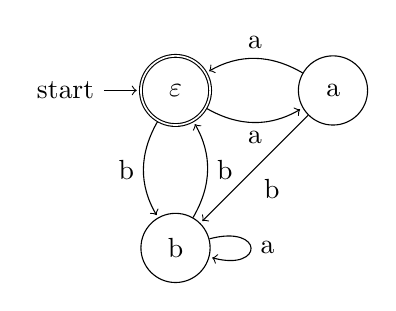
\begin{tikzpicture}[shorten >=1pt,node distance=2cm,on grid,auto] 
 \node[state,initial,accepting] (s_0) {$\varepsilon$};
 \node[state] (s_a)[right=of s_0] {a};
 \node[state] (s_b)[below=of s_0] {b};
 \path[->] 
 (s_0) edge [bend right,below] node {a} (s_a)
 (s_0) edge [bend right,left] node {b} (s_b)
 (s_a) edge [bend right,above] node {a} (s_0)
 (s_a) edge [bend right=0,below right] node {b} (s_b)
 (s_b) edge [bend right,right] node {b} (s_0)
 (s_b) edge [loop right] node {a} (s_b);
\end{tikzpicture}
 \end{document}